\documentclass[a4paper]{article}
\usepackage{lipsum}
\usepackage{graphicx,subcaption}

\begin{document}
\lipsum[1]

\begin{figure}[h!]
\def\CE{0.24}
\centering
\begin{subfigure}[b]{\CE\textwidth}
    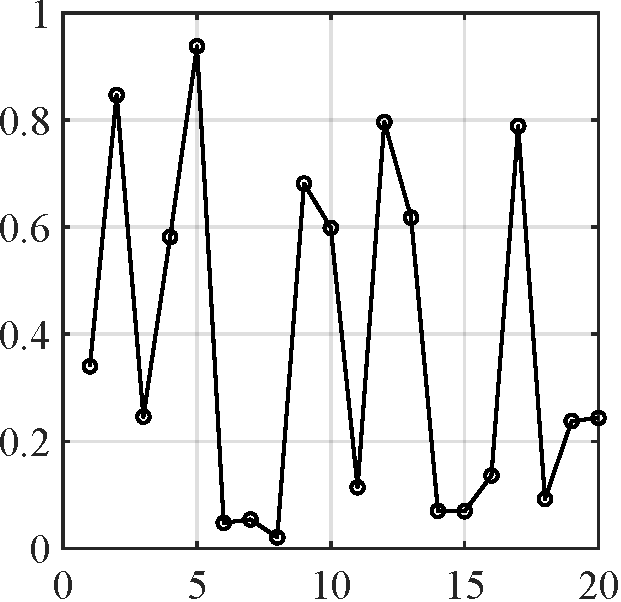
\includegraphics[width=\textwidth]{pic-1.pdf}
    \caption{Data series A.}
    \label{fig-a}
\end{subfigure}
\hfill
\begin{subfigure}[b]{\CE\textwidth}
    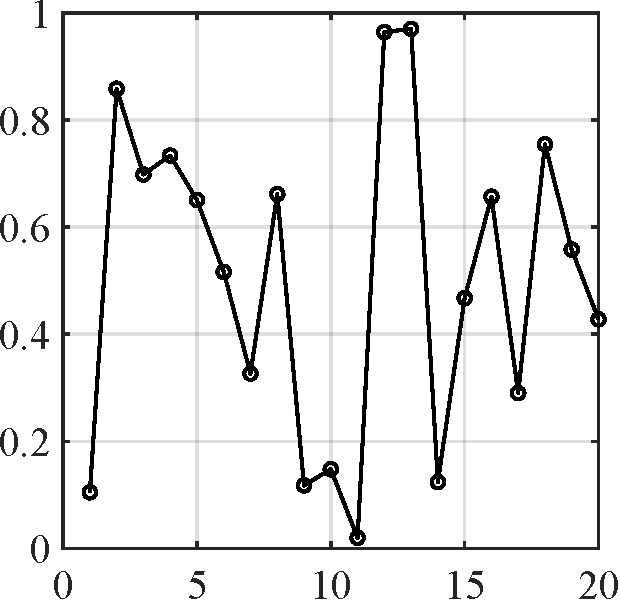
\includegraphics[width=\textwidth]{pic-2.pdf}
    \caption{Data series B.}
    \label{fig-b}
\end{subfigure}
\hfill
\begin{subfigure}[b]{\CE\textwidth}
    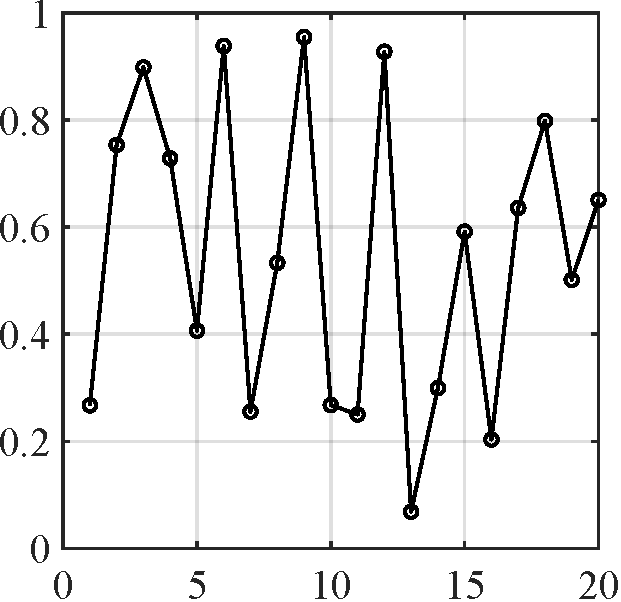
\includegraphics[width=\textwidth]{pic-3.pdf}
    \caption{Data series C.}
    \label{fig-c}
\end{subfigure}
\hfill
\begin{subfigure}[b]{\CE\textwidth}
    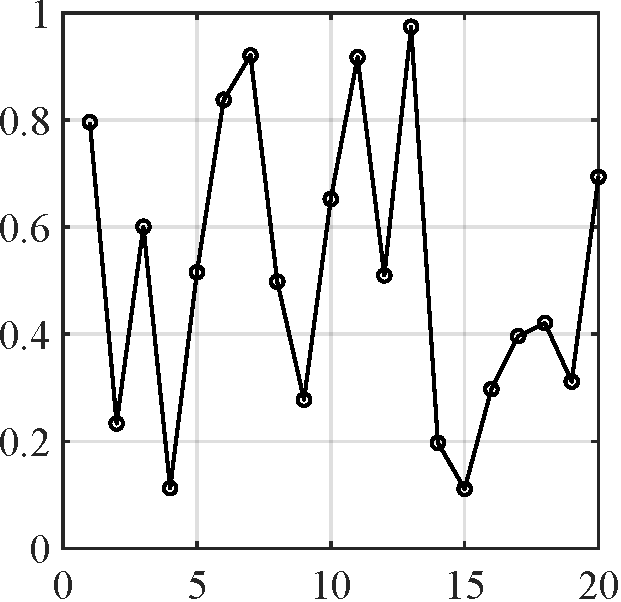
\includegraphics[width=\textwidth]{pic-4.pdf}
    \caption{Data series D.}
    \label{fig-d}
\end{subfigure}\\
\begin{subfigure}[b]{\CE\textwidth}
    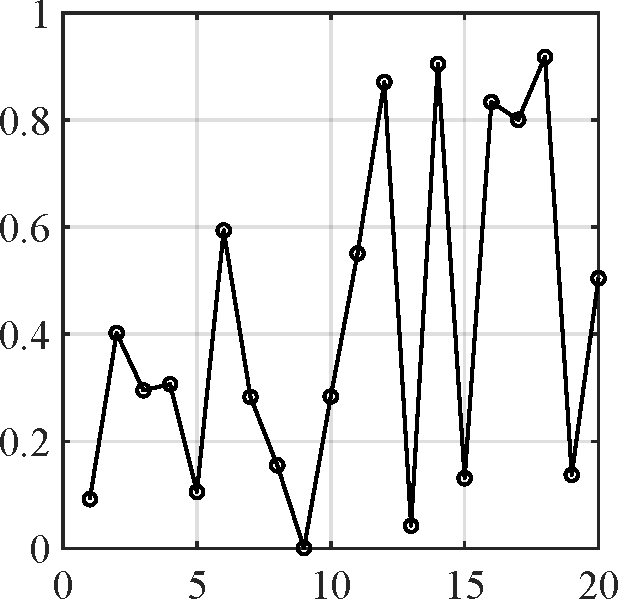
\includegraphics[width=\textwidth]{pic-5.pdf}
    \caption{Data series E.}
    \label{fig-e}
\end{subfigure}
\hfill
\begin{subfigure}[b]{\CE\textwidth}
    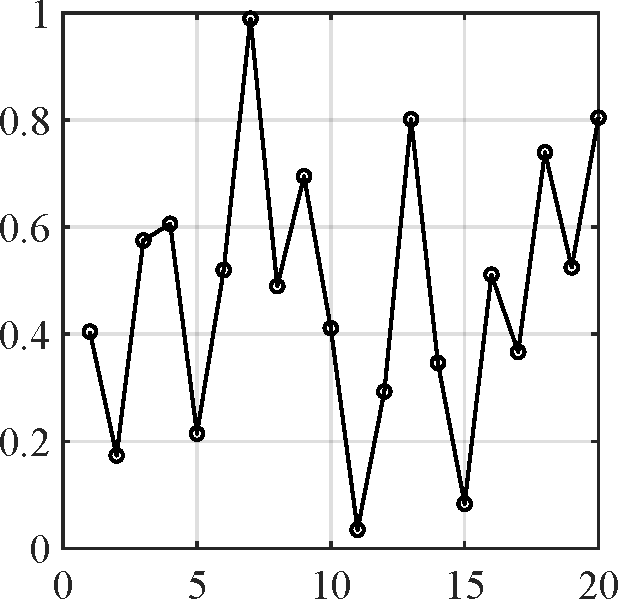
\includegraphics[width=\textwidth]{pic-6.pdf}
    \caption{Data series F.}
    \label{fig-f}
\end{subfigure}
\hfill
\begin{subfigure}[b]{\CE\textwidth}
    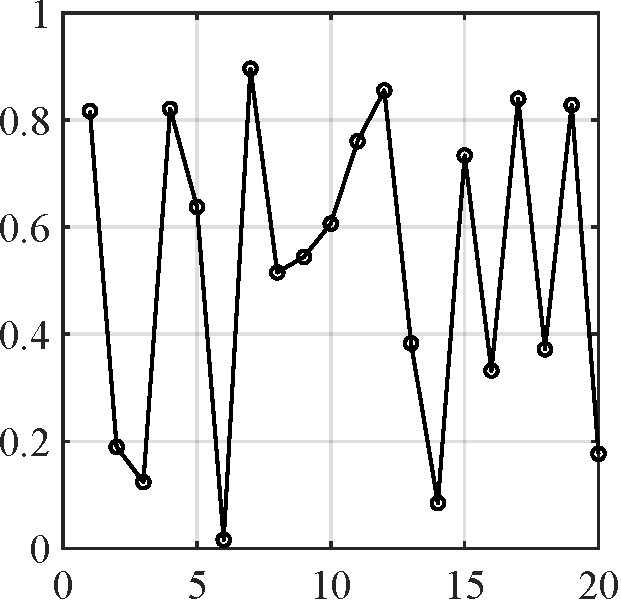
\includegraphics[width=\textwidth]{pic-7.pdf}
    \caption{Data series G.}
    \label{fig-G}
\end{subfigure}
\hfill
\begin{subfigure}[b]{\CE\textwidth}
    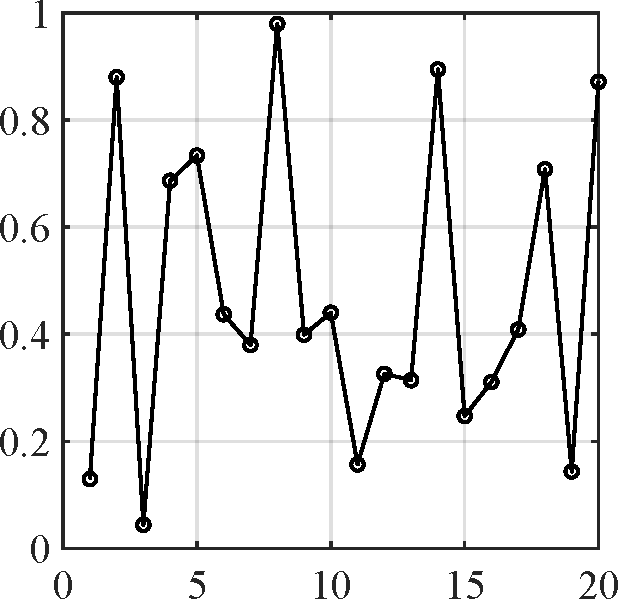
\includegraphics[width=\textwidth]{pic-8.pdf}
    \caption{Data series H.}
    \label{fig-H}
\end{subfigure}
\caption{This is caption.}
\label{fig}
\end{figure}

This is Fig. \ref{fig}, and this is subfigure Fig. \ref{fig-a}.

\end{document}